\subsection{Target Group - Fishing Enthusiasts}
\label{TargetGroup}
\begin{wrapfigure}{r}[15pt]{0.35\textwidth}
\vspace{-\baselineskip}
\centering
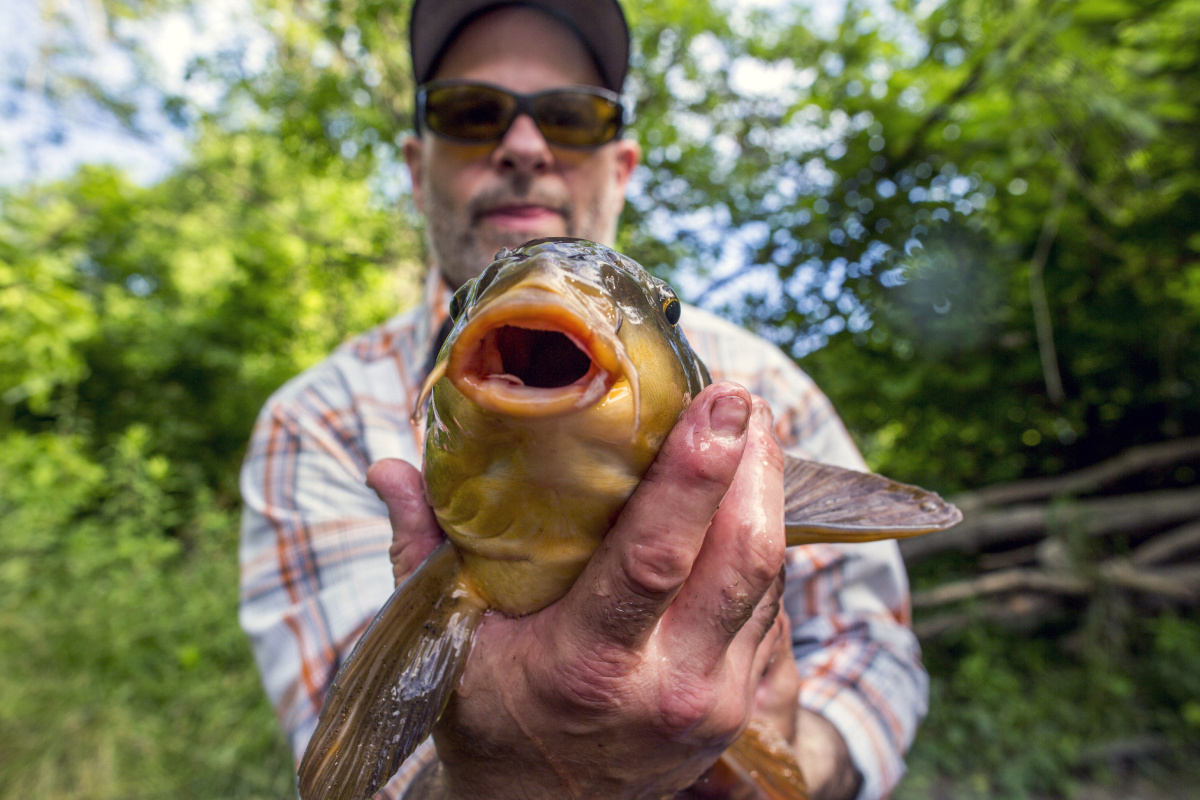
\includegraphics[width=0.35\textwidth]{Img/FishingEnthusiast}
\caption{Fishing Enthusiast.}
\end{wrapfigure} 
The main purpose of the application is to bring closer people living in the area, mainly those that are fishing pros and people who come to the area because of fishing and other similar activities in the nature, everything to the economic benefit of locals without damaging the already fragile environment. It is expected that it could also attract new people unaware of the region to visit the area. 
Since we decided to focus on fishing aspect, our target group are \textbf{fishing enthusiasts}, which can actually be divided into two different groups:
\begin{itemize}
\item Locals.
\item Tourists.
\end{itemize}
\subsubsection{Their needs}
\paragraph*{Locals} need a new income system, something new that could bring jobs and opportunities in the area using
the natural environment of the zone such as the river and the woods that follow the Elk River.
\paragraph*{Tourists} coming from other counties want instead a different experience, somewhere new where
they can fish different species and enjoy a new area different from the ones they usually go to.
\subsubsection{What are we offering them?}
A service that will facilitate the organization and the building of an infrastructure for fishing enthusiasts using
modern technologies, this would create new job opportunities (such as local guides, fishing instructors,
boat rentals, ecc...) for the locals and allow tourists to easily come to the Elk River and enjoy
a weekend without the stress of organizing everything by themselves.
\subsubsection{Other information}
\paragraph*{How many are there?} About 1.5Million.
\paragraph*{How many will we reach?} Around 50.000 people.
\paragraph*{How frequently will we interact with them?} Weekly.
\paragraph*{What do we get in return?} Economic growth.
\paragraph*{How can our relationship grow?} With people talking about the service.
\clearpage
\subsection{Personas}
\subsubsection{Bob The Fishing Enthusiast}
\begin{wrapfigure}{r}[15pt]{0.3\textwidth}
\vspace{-\baselineskip}
\centering
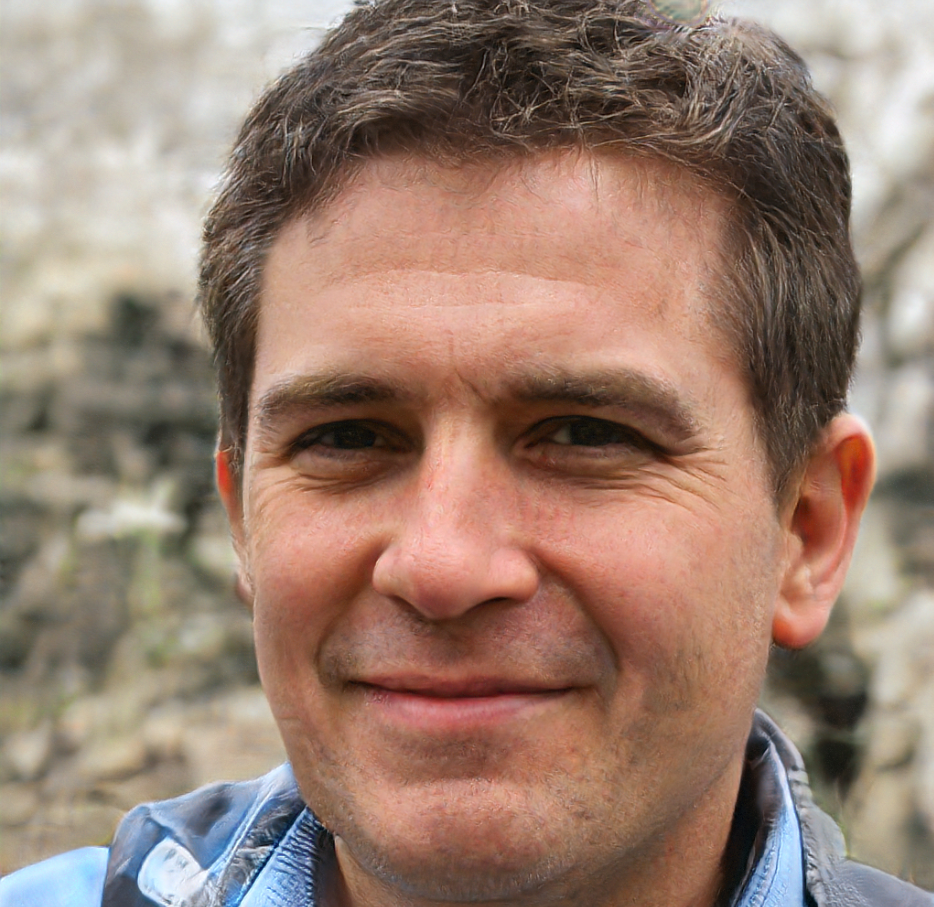
\includegraphics[width=0.3\textwidth]{Img/Bob}
\caption{Bob the local.}
\vspace{-2cm}
\end{wrapfigure} 
\paragraph*{Who is Bob?}
Bob (40) is father of 2 young children (10 and 12) and has lived his entire life in the small town (700 people) of Webster Springs West Virginia. He used to work at Freedom Industries before the spill of 2014 when shortly after the company filed for bankruptcy and Bob was left without a job. Given that he never attended college and the little possibilities in his hometown, Bob now works at his wife's bakery while he is still searching for another job to help the family put aside some money for the children tuition and health care plan.
\paragraph*{His interests:}
Interests: Fishing, camping, hiking, restoring classic cars and classical music. 
\paragraph*{Reasons for him to engage with us:}
He is looking for a new job, knows the territory and believes it can be used for tourism and fishing enthusiasts like himself, has been fishing all his life and would love to teach people how to fish.
\paragraph*{Reasons for him NOT to engage with us:}
He isn't sure it would provide enough for his family the water is still not completely clean, too many tourists may destroy the natural environment of the area.
\paragraph*{His skills:}
Fishing expert, Great sense of direction, it's almost impossible for him to get lost in the local area he has been roaming since childhood, good survival skills, basic medical training, he can also cook the best trout on the grill of the state.
\paragraph*{His typical day:}
Bob wakes up with his wife every weekday at 4:40 AM and they both head up to the bakery in order to prepare everything the little community needs during the day. At around 7:00 AM he takes the little van they have for the activity and starts the delivery for the other businesses of the area and once he is done he goes back home to work on his latest car project until he has to go and pick up the kids from school. Once home again, they eat all together and then he watches some baseball with the kids before helping then with their homework until it's time for dinner. After the boys are in bed he likes to relax for some time on his chair listening to some classical music before going to bed himself, always waiting for the next fishing trip during the weekend.
\paragraph*{His personality:}
Bob is a kind man that always has a smile on his face, no matter the situation. He is an optimist at heart and always believes that everything will be alright and no problem can't be solved if people work together. He is always the first one to volunteer when work for the community has to be done and takes pride and joy in helping the others when they are in need, often refusing any form of compensation. 
\paragraph*{His social environment:}
Active member of the community in the small town of Webster Springs West Virginia he is well known and respected. He's usually more forward thinking than the older people that live in town and since he is more accepting of new ideas for the future he often can convince the others to back up new opportunities. 
\paragraph*{His dreams:}
Have an independent job, spend more time with his kids, provide more for his family, buy a 1968 Mustang and then restore it with his children
\clearpage
\subsubsection*{Jack The Tourist Fisherman}
\begin{wrapfigure}{r}[15pt]{0.3\textwidth}
\vspace{-\baselineskip}
\centering

\includegraphics[width=0.3\textwidth]{Img/Jack}
\caption{Jack the tourist.}
\vspace{-1.5cm}
\end{wrapfigure}
\paragraph*{Who is Jack?}
Jack(36) is a father of a little girl (6 years) and lives with her and his wife in Columbus, Ohio. He is an IT technician in a medium size company where he has been working since 2007 and is a respected employee. He never obtained a degree but studies IT in high school and has always been tech savvy. Jack's father always brought him to do outdoors activities when he was younger, from rafting to camping, he always loved playing football until he got a knee injury, but his true passion has always been fishing, which he does to this day with his father and friend. 
\paragraph*{His interests:}
Fishing, camping, driving, football, rafting and bowling.
\paragraph*{Reasons for him to engage with us:}
He wants a new place to spend the weekend fishing, even though he knows how to fish the "usual" way he never tried fly fishing and would like to try, he also loves natural places and off the grid camping spots.
\paragraph*{Reasons for him NOT to engage with us:}
He's never been to West Virginia, he knows of the spill and still doesn't trust the area after it and it's a longer drive than usual. 
\paragraph*{His skills:}
Fishing expert, tech enthusiast, problem solver, knows his way in the great outdoors.
\paragraph*{His typical day:}
Jack wakes up every weekday at 7:00 AM with the family, they all have breakfast together and then he brings his daughter to preschool and then goes to work which starts at 8:00 AM. Around 12:30 AM he heads back home for lunch, which he usually prepares when his wife arrives home with the little girl. After lunch he helps his daughter to bed for the afternoon nap and heads back to work for the afternoon shift. Once home again in the evening they have dinner and spend some more time together watching some TV until it's bedtime for the kid, once she is asleep Jack usually caches up with the latest football updates until it's time for him too to go to sleep. 
\paragraph*{His personality:}
Jack is a loving father and husband, a great friend and he is know at work for his great work ethic. He rarely gets upset and is always glad to learn something new, from a simple fact, to a new tech that is going to change the marker, up to a better way to do his job. He worked for what he has but does not like to remind people of this and is a great teacher, whether it is on the job, at the bowling alley or during a fishing trip with someone new joining the group.  
\paragraph*{His social environment:}
One of the most experienced people in the company he works for and between the ones that have been there since the early years, Jack is well known and respected by his colleagues and loved by his friends. He is always present at every social event, from birthdays to a quite evening in the bar. 
\paragraph*{His dreams:}
Become a manager of the company, teach his daughter to fish, buy a house with a pond.
